\documentclass[12pt,a4paper]{report}
\usepackage[utf8]{inputenc}
\usepackage{graphicx}
\usepackage{geometry}
\usepackage{setspace}
\usepackage{titlesec}
\usepackage{amsmath}
\usepackage{float}

% Chapter Header Refinement
\titleformat{\chapter}[display]
  {\normalfont\huge\bfseries}{CHAPTER \thechapter}{10pt}{\Huge}
\titlespacing*{\chapter}{0pt}{10pt}{20pt} % Standard academic top spacing

\geometry{top=1in, bottom=1in, left=1.25in, right=1in}
\setstretch{1.5} % 1.5 line spacing typical for academic reports

\begin{document}

% -------------------------
% TITLE PAGE
% -------------------------
\begin{titlepage}
    \begin{center}
        \textbf{\Large Lincoln University College}\\
        \textbf{\large Faculty of Computer Science and Multimedia}\\
        
        \vspace{1.5cm}
        
        \textbf{\LARGE Defend \& Detect:}\\
        \textbf{\LARGE AI-Powered Cybersecurity Platform}\\
        
        \vspace{1.5cm}
        
        \textbf{A PROJECT REPORT}\\
        \vspace{0.5cm}
        Submitted to\\
        \textbf{Department of Information Technology}\\
        \textbf{Phoenix College of Management}\\
        Maitidevi, Kathmandu\\
        
        \vspace{1.5cm}
        
        In partial fulfillment of the requirements for the\\
        \textbf{Bachelor in Information Technology (BIT)}\\
        
        \vspace{1.5cm}
        
        Submitted by\\
        \textbf{Sabinesh Rajbhandari}\\
        BIT 7th Semester\\
        University ID: LC0003001698\\
        
        \vfill
        
        \textbf{2026/03}
    \end{center}
\end{titlepage}

% -------------------------
% DECLARATION & APPROVAL
% -------------------------
\newpage
\begin{center}
    \textbf{\LARGE Declaration}
\end{center}
\addcontentsline{toc}{section}{Declaration}

I hereby declare that the project report entitled \textbf{``Defend \& Detect: AI-Powered Cybersecurity Platform''} is my original work, completed under the guidance of Mr. Saishab Bhattarai. This report has not been submitted elsewhere, in full or in part, for the award of any degree, diploma, or other academic recognition.

\vspace{0.8cm}

\noindent
\textbf{Name:} Sabinesh Rajbhandari \\
\textbf{Signature:} \rule{5cm}{0.4pt} \\
\textbf{Date:} 2026/03/ \rule{2cm}{0.4pt}

\vspace{1.5cm}

\newpage
\begin{center}
    \textbf{\Large Lincoln University College}\\
    \textbf{\large Faculty of Computer Science and Multimedia}\\
    \textbf{Phoenix College of Management}\\
    Maitidevi, Kathmandu\\
    \textbf{Bachelor in Information Technology (BIT)}
\end{center}

\vspace{0.5cm}

\begin{center}
    \textbf{\LARGE LETTER OF APPROVAL}
\end{center}
\addcontentsline{toc}{section}{Letter of Approval}

The project report entitled \textbf{``Defend \& Detect: AI-Powered Cybersecurity Platform''}, submitted by \textbf{Sabinesh Rajbhandari} (University ID: LC0003001698), in partial fulfillment of the requirements for the Bachelor’s degree in Information Technology, has been accepted as a record of work independently carried out under the guidance of the department.

\vspace{0.5cm}
In our opinion, it is satisfactory in the scope and quality of the project for the required degree.

\vspace{2cm}

\noindent
\begin{minipage}{0.45\textwidth}
    \rule{6cm}{0.4pt}\\
    \textbf{Er. Santosh Dhungana}\\
    Head of Department
\end{minipage}
\hfill
\begin{minipage}{0.45\textwidth}
    \rule{6cm}{0.4pt}\\
    \textbf{Mr. Saishab Bhattarai}\\
    Internal Examiner
\end{minipage}

\vspace{2cm}

\noindent
\begin{minipage}{0.45\textwidth}
    \rule{6cm}{0.4pt}\\
    \textbf{Mr. Bijay Mishra}\\
    Program Coordinator
\end{minipage}
\hfill
\begin{minipage}{0.45\textwidth}
    \rule{6cm}{0.4pt}\\
    \textbf{External Examiner}\\
\end{minipage}

% -------------------------
% CERTIFICATE
% -------------------------
\newpage
\chapter*{Certificate}
\addcontentsline{toc}{chapter}{Certificate}

This is to certify that the project report entitled \textbf{“Defend \& Detect: AI-Powered Cybersecurity Platform”}, submitted by \textbf{Sabinesh Rajbhandari} (University ID: LC0003001698) to Lincoln University College in partial fulfillment of the requirements for the Bachelor in Information Technology, is a record of original work carried out under my supervision and guidance.

\vspace{2cm}

\noindent
\textbf{Supervisor Name:} Mr. Saishab Bhattarai \\
\textbf{Designation:} Project Coordinator \\
\textbf{Signature:} \rule{5cm}{0.4pt} \\

% -------------------------
% ABSTRACT
% -------------------------
\newpage
\chapter*{Abstract}
\addcontentsline{toc}{chapter}{Abstract}

The \textbf{Defend \& Detect Platform} is designed to assist end-users, students, and organizations in maintaining digital security by identifying malicious artifacts and obfuscated threats. By automatically detecting potential phishing attempts, suspicious URLs, and zero-day vulnerabilities, the system provides a reliable, all-in-one methodology for evaluating cybersecurity risks.

The system analyzes raw text and network input, applies advanced detection algorithms including Lexical Entropy, YARA pattern matching, and Deep Learning Transformers (BERT), and generates comprehensive reports using a Large Language Model (Llama 3). This tool streamlines the threat review process, eliminates the need to navigate multiple fragmented security tools, and promotes deeper educational understanding of cyber attacks.

\vspace{0.5cm}
\noindent
\textbf{Keywords:} Threat Detection, Cybersecurity, Artificial Intelligence, Lexical Analysis, Vulnerability Verification, Language Models.

% -------------------------
% TABLE OF CONTENTS
% -------------------------
\newpage
\tableofcontents
\newpage

% -------------------------
% MAIN CONTENT CHAPTERS
% -------------------------

\chapter{Introduction}
\section{Introduction}
The global digital landscape is facing an unprecedented surge in sophisticated cyber threats, ranging from polymorphic malware and AI-driven phishing to zero-day vulnerabilities in critical infrastructure. The democratization of "Phishing-as-a-Service" (PhaaS) and the shift from traditional signature-based detection to AI-native behavioral analysis has increased the sheer volume and nuance of these attacks. While professional security tools exist, they are often fragmented and produce highly technical output that is inaccessible to non-expert users or students. There is a critical need for a unified, intuitive platform—\textbf{Defend \& Detect}—that bridges the gap between high-end forensic telemetry and user-centric education, providing human-readable explanations of the underlying attack mechanics to reduce the window of exploitation.

\section{Problem Statement}
Current cybersecurity analysis is hindered by ``Technical Information Overload,'' where users are overwhelmed by raw forensic data without contextual guidance. Analysts typically face a ``swivel-chair'' effect, having to jump between multiple disjointed web consoles (VirusTotal, NVD, WHOIS, etc.) to evaluate a single threat. Furthermore, the ``Expert Gap'' means that raw JSON/CSV outputs from security APIs are meaningless to BIT students or small business owners without a localized reasoning layer. Existing automated scanners often act as ``Black Boxes''---providing a ``Malicious'' score without educating the user on \textit{why} or \textit{how} the attack functions, which prevents long-term defensive learning and institutional resilience.

\section{Objectives}
The primary objective of this project is to develop and deploy an AI-Powered Cybersecurity Platform—\textbf{Defend \& Detect}—that centralizes forensic intelligence into a single, accessible web interface.
Specific objectives include:
\begin{enumerate}
    \item \textbf{Phishing Analysis:} Utilize Deep Learning (BERT) to identify semantic deception in raw text.
    \item \textbf{URL Intelligence:} Automate reputation scoring via VirusTotal, WHOIS, and GeoIP lookup.
    \item \textbf{Vulnerability Translation:} Query the NVD API and use Llama 3 to translate complex CVEs into plain-English.
    \item \textbf{Forensic Data Persistence:} Implement a localized history using SQLite for long-term threat tracking.
\end{enumerate}

\section{Scope and Limitation}
The platform is designed as an investigative and educational cybersecurity workbench. While it provides high-fidelity analysis of point-in-time artifacts (emails, URLs, logs), it is not intended to function as a real-time Antivirus, Firewall, or active Endpoint Detection and Response (EDR) agent.

\section{Development Methodology}
The project employs an \textbf{Agile / Prototyping} methodology, ensuring the modular delivery of forensic services through iterative sprints. Each sprint focuses on a specific detection module (Phishing $\rightarrow$ URL $\rightarrow$ CVE $\rightarrow$ LLM synthesis), allowing for rapid refinement and user-centric UI adjustments.

\section{Report Organization}
This report is organized into four core chapters: \textbf{Chapter 1: Introduction} (Overview and Goals), \textbf{Chapter 2: Background Study} (Theoretical Foundation and Literature Review), \textbf{Chapter 3: System Analysis \& Design} (UML Modeling and Requirements), and \textbf{Chapter 4: Conclusion} (Summary and Future Scope).

% -------------------------
\chapter{Background Study and Literature Review}

\section{Background Study}
The \textbf{Defend \& Detect} platform leverages a modern technical stack to solve the fragmentation problem. The core analytical logic utilizes the \textbf{Python} ecosystem for rapid data processing, \textbf{Streamlit} for a reactive and prestigious UI, and high-fidelity API integrations including \textbf{Hugging Face} (Deep Learning models), \textbf{Groq/Llama 3} (Generative AI logic), and \textbf{NVD/VirusTotal} (Deterministic intelligence).

\section{Literature Review}
Phishing email detection has been extensively studied to determine the effectiveness of advanced pattern recognition. Latha et al. [1] conducted an analysis of phishing models, emphasizing the importance of deep learning techniques, specifically transformer models like BERT. They noted that traditional keyword filters often fail to detect cleverly obfuscated semantic intent, and deep learning approaches yield significantly higher detection accuracy.

Aljabri et al. [2] reviewed existing machine learning techniques for detecting malicious URLs, analyzing their applicability against evolving zero-day threats. The study highlighted that while basic algorithmic models excel in identifying structured similarity, they may fall short in handling highly dynamic command-and-control infrastructure, underscoring the need for hybrid systems that combine lexical analysis with active threat intelligence.

Similarly, Latha et al. [3] provided an overview of API-based malware verification, indicating that leveraging aggregate engines like the VirusTotal API significantly increases detection capabilities. The study further emphasized that automating SHA-256 hash scanning against multiple security vendors simultaneously reduces false positives and provides deterministic intelligence for security analysts.

Shahzad et al. [4] examined vulnerability management frameworks, noting that systematic analysis of the National Vulnerability Database (NVD) is crucial for evaluating actual exploitation risk. Even with CVSS scoring, automated API integration is required to accurately filter, prioritize, and translate technical CVE data for timely patch management and infrastructure defense.

Finally, Jiang et al. [5] compared traditional log parsing methods with modern Generative AI and concluded that Large Language Models (LLMs) dramatically improve system efficiency and report comprehensiveness. The study emphasized that LLMs can adaptively translate unstructured server errors into actionable insights without the need for rigid, pre-defined regex rules.

Overall, our project builds upon these theoretical foundations to offer an integrated, reliable solution for both educators and security professionals alike.

% -------------------------
\chapter{System Analysis and Design}

\section{System Analysis (Object-Oriented Approach)}
\subsection{Requirement Analysis}
\textbf{i. Functional Requirements (FR):}
\begin{itemize}
    \item \textbf{FR1: Phishing Analysis:} The system shall process raw text via Hugging Face BERT and Groq LLM synthesis to identify deceptive intent.
    \item \textbf{FR2: URL Reputation Scan:} The system shall deconstruct URLs to extract WHOIS, GeoIP, and aggregate VirusTotal reputation findings.
    \item \textbf{FR3: CVE Intelligence:} The system shall query the NVD API for vulnerability metadata and translate complex CVE records into plain-English insights.
    \item \textbf{FR4: Comparison Engine:} The system shall allow users to perform a visual, side-by-side comparison of two historical threat payloads.
    \item \textbf{FR5: Forensic Logging:} The system shall automatically persist all scan telemetry to a localized SQLite history for future forensic review.
\end{itemize}

\textbf{ii. Non-Functional Requirements (NFR):}
\begin{itemize}
    \item \textbf{NFR1: Performance:} All external API orchestrations must resolve or gracefully timeout within 15 seconds to ensure a responsive dashboard.
    \item \textbf{NFR2: Security:} The system shall strictly sanitize all inputs using HTML escaping and utilize parameterized SQL queries to prevent XSS and SQLi.
    \item \textbf{NFR3: Usability:} The platform must be mobile-responsive, utilizing sidebars and vertical stacking for seamless on-the-go analysis.
\end{itemize}

\subsection{Functional Analysis: Use Case Diagram}
The functional analysis illustrates the interaction between the primary actor (Security Analyst) and the system's specialized forensic modules. This diagram defines the platform boundary and maps the specific external interfaces (e.g., Hugging Face, VirusTotal, Groq) required for automated analysis.

\begin{figure}[H]
    \centering
    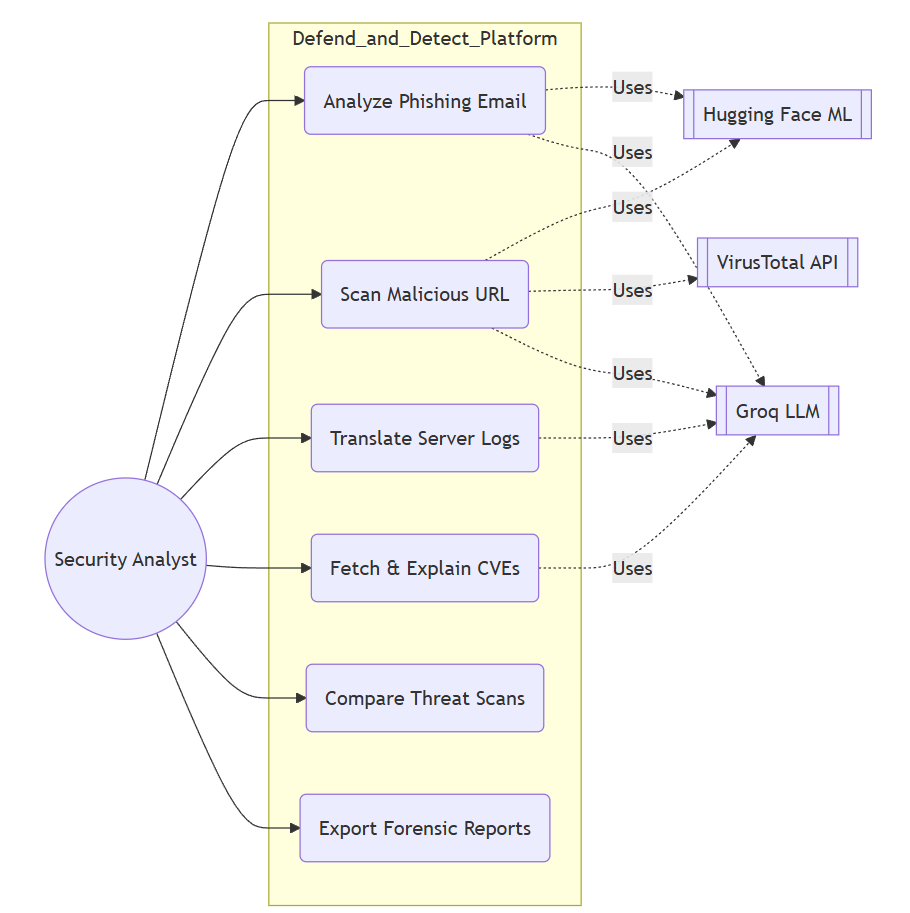
\includegraphics[width=0.85\textwidth]{images/use_case_diagram.png}
    \caption{Use Case Diagram modelling System Functionalities}
\end{figure}

\subsection{Feasibility Analysis}
The project feasibility is evaluated across four core professional dimensions:
\begin{enumerate}
    \item \textbf{Technical Feasibility:} The platform utilizes the robust Python ecosystem (Streamlit) for rapid UI development and integrates enterprise-grade, well-documented APIs (Groq, Hugging Face, VirusTotal). The modular service-oriented architecture ensures technical complexities are isolated and manageable.
    \item \textbf{Operational Feasibility:} There is a significant academic demand for consolidated, educational cybersecurity tools. The platform is designed to be intuitive for both students and security professionals, making it highly viable for real-world investigative environments.
    \item \textbf{Economic Feasibility:} By leveraging open-source libraries and the free-tier availability of industry-leading APIs, the project minimizes operational overhead costs, ensuring total cost-effectiveness and sustainability.
    \item \textbf{Schedule Feasibility:} Adopting an Agile / Prototyping methodology allows for the delivery of core forensic modules in incremental sprints, ensuring all key objectives are successfully met within the academic timeline.
\end{enumerate}

\subsection{Object Modelling: Class Diagram}
The architecture involves distinct services decoupled from the UI: \texttt{DatabaseService}, \texttt{IntelligenceService}, and \texttt{GroqService}.

\begin{figure}[H]
    \centering
    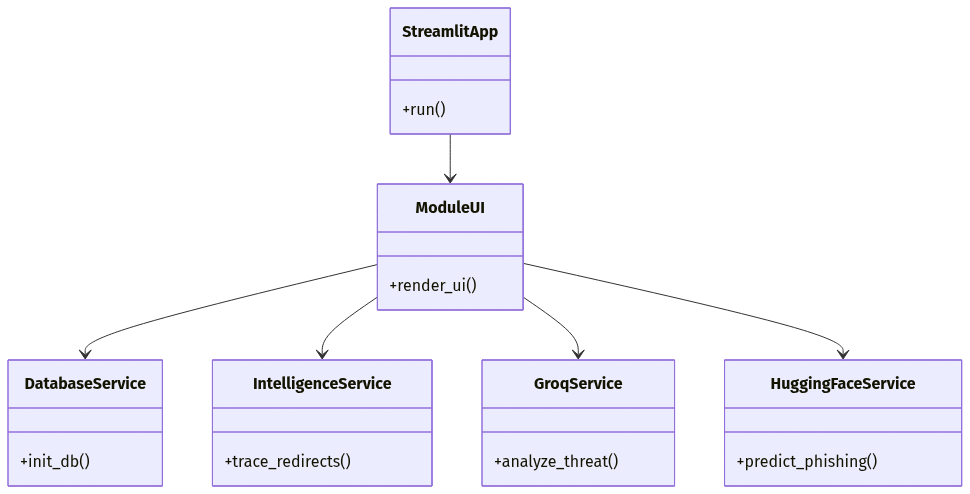
\includegraphics[width=1.1\textwidth]{images/class_diagram.png}
    \caption{Class Diagram representing Object Modelling}
\end{figure}

\subsection{Dynamic Modelling: Sequence Diagram}
The dynamic modelling of the platform illustrates the end-to-end lifecycle of a threat analysis request. The workflow begins at the \textbf{UI Layer}, which captures raw input and transmits it to the \texttt{IntelligenceService}. This service facilitates concurrent analysis by querying local \texttt{YARA} engines and remote \texttt{Threat-Intel APIs} (e.g., VirusTotal).

The gathered telemetry is then synthesized by the \texttt{GroqService}, leveraging Large Language Models (LLMs) to provide human-readable risk assessments. The final results are asynchronously persisted via the \texttt{DatabaseService} to ensure historical visibility before being rendered on the user's dashboard.

\begin{figure}[H]
    \centering
    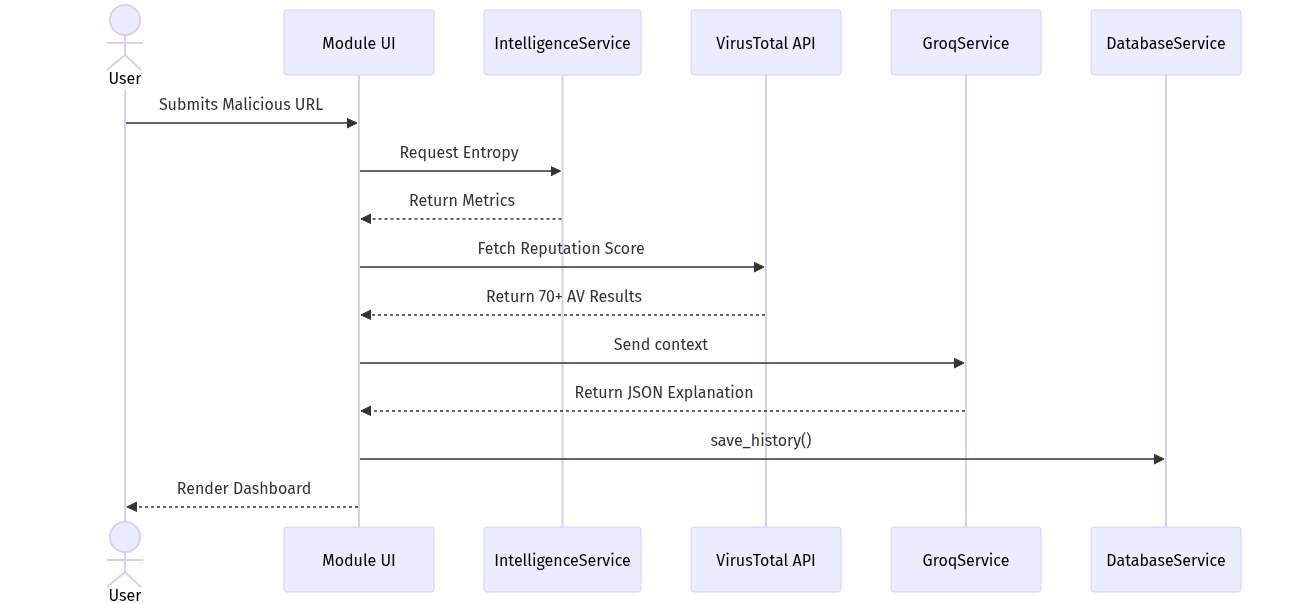
\includegraphics[width=1.1\textwidth]{images/sequence_diagram.png}
    \caption{Sequence Diagram modelling the Threat Scan Workflow}
\end{figure}

\subsection{Process Modelling: Activity Diagram}
The activity diagram captures the procedural logic and concurrency of the platform. The process begins from an \textbf{Idle} state, where the system monitors for user-initiated scan requests. Once active, the flow transitions into a mandatory \textbf{Input Validation} lock, ensuring that only sanitized strings move forward to the operational core.

Post-validation, the system employs a \textit{fork} to execute \textbf{Parallel Intelligence Gathering}—simultaneously querying local \texttt{YARA} signatures and remote threat-intel telemetry (e.g., VirusTotal). These disparate logical paths \textit{join} at the \textbf{AI Reasoning Engine}, where a Large Language Model synthesizes the findings. The finalized report is then persisted to the \texttt{DatabaseService} and rendered on the user dashboard, returning the system to its baseline idle state.

\begin{figure}[H]
    \centering
    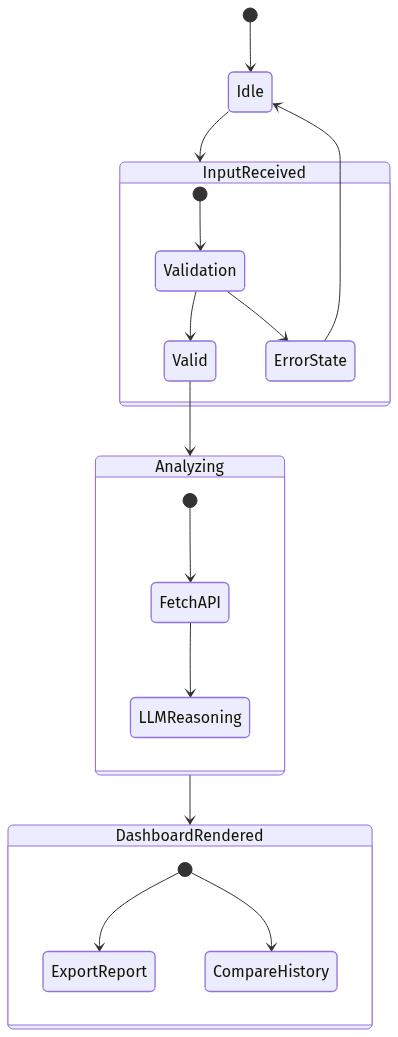
\includegraphics[width=1.1\textwidth,height=0.55\textheight,keepaspectratio]{images/activity_diagram.png}
    \caption{Activity Diagram modelling user and system processes}
\end{figure}

\section{System Design}
\subsection{Refinement of Classes and Objects}
Strict adherence to single-responsibility isolates database transactions from network I/O calls to prevent bloated architecture.

\subsection{Component Diagram}
The physical architecture is structured into three meticulously delineated layers:
1. \textbf{Presentation Layer:} The dynamic Streamlit Web UI.
2. \textbf{Logic Layer:} The core analytical engine handling forensic math.
3. \textbf{Data Layer:} The localized SQLite storage infrastructure.

\begin{figure}[H]
    \centering
    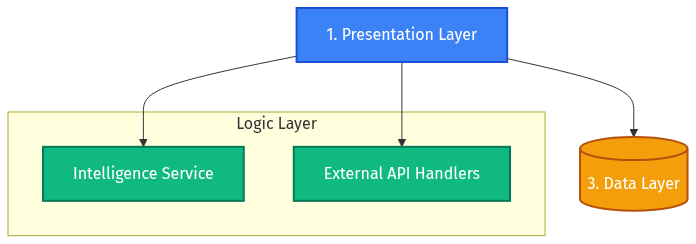
\includegraphics[width=0.85\textwidth,height=0.25\textheight,keepaspectratio]{images/component_diagram.png}
    \caption{Component Diagram of Physical Architecture}
\end{figure}

\subsection{Deployment Diagram}
The application supports containerized encapsulation (Docker) navigating outward via encrypted HTTPS to interact with external Intelligence ecosystems.

\begin{figure}[H]
    \centering
    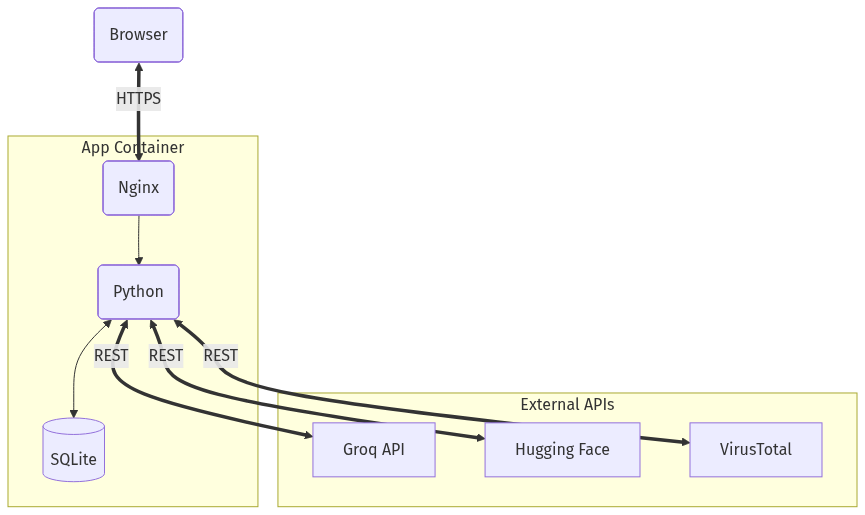
\includegraphics[width=1.1\textwidth,height=0.4\textheight,keepaspectratio]{images/deployment_diagram.png}
    \caption{Deployment Diagram of Cloud integration}
\end{figure}

\clearpage
\section{Algorithm Details}
\textbf{Lexical Analysis (Shannon Entropy):}
This algorithm mathematically quantifies the inherent randomness of characters within a given string: $H(X) = - \sum (p_i \times \log_2(p_i))$. Legitimate URLs exhibit structural predictability, whereas malicious domains yield exceptionally high entropy.

- \textbf{Supervised ML Classification (BERT):} Utilizes pre-trained transformer weights via Hugging Face to process the sentiment and syntax of an email string, outputting a normalized confidence score (0.0 to 1.0) indicating malicious probability.

- \textbf{YARA Pattern Matching:} A deterministic Boolean algorithm (`1` or `0`) that scans text against a local compilation of byte-level and string-level rules (\texttt{phishing.yar}) to enforce rigid, non-AI based security confirmations.

\end{document}
